\chapter{Methodology}
\label{chap:methods}
Four separate stages of this thesis can be defined: data acquisition (guitar recording), transcription, feature extraction and models computation. Expressive hexaphonic guitar recordings will be done using the Roland GK-3 divided pick-up, which is able to separate sound from each string~\cite{Angulo2016}. The main output of this first stage will be a new dataset consisting of hexaphonic recordings recorded by a professional guitar player with different performance actions of the performance depending on a given mood. \\
After this step, transcription of each individual string will be computed applying non-negative matrix factorization~\cite{OGrady2009}. After doing a score alignment with the original score and the transcription of the expressive guitar performance, feature extraction needs to be done.\\
Feature extraction will be performed following an approach in which each note is characterized by its \textit{nominal}, \textit{neighbouring}, and \textit{contextual} properties.  Here is where the most of the research in this thesis will take place:  checking for literature in expressive piano modelling, combining it with previously mentioned features of monophonic expressive guitar modelling,... \\
Several machine learning and feature selection algorithms will be applied to predict those performance actions (timing, pitch, energy,...) and ornaments introduced by the musician when performing a musical piece.


\section{Data acquisition}
In order to obtain hexaphonic recordings and get each string nicely separated we used the Roland GK-3 divided pickup that is easily attached to any steel-stringed electric guitar and acts as a sound transduction device. It is able to separate very good the sound from each string and delivers accurate performance data. \\
However, the output of this pickup consists of a 13 pin DIN cable that allows to connect the guitar to guitar synthesizers such as Roland's popular GR-55 and at the same time to fed electrically the pickup. So, in order to be able to record each string separately we need to adapt the pickup output so the sound of each string can be inputted to the computer through an independent input chanel of an audio interface.\\
To do this, a Breakout Box circuit was built by I.Angulo~\cite{Angulo2016} for his master's thesis last year so we reused it. The final box has an input for the 13 pin DIN cable and 6 separate Jack connector cables are outputted, one for each string. Also, two batteries are needed inside the box in order to fed the pickup.



\section{Hexaphonic guitar transcription}


\section{Feature extraction}
\begin{table}[ht!]
\centering
  \caption[Chord description.] {Chord description. A list of chords definitions.  The numbers on the Intervals column indicate the index of the notes belonging to the chord, (zero indexed, in 12 semitones).}
  \label{tab:chord_extensions}
  \begin{tabular}{  l  c  l }
    \hline
    Chord type & Intervals & Example (C as root) \\ \hline
    M (major) & 0 4 7 & C E G \\
    m (minor) & 0 3 7 & C E$\flat$ G \\
    2 (sus2) & 0 2 7 & C D G \\
	sus (sus4) & 0 5 7 & C F G \\
    dim & 0 3 6 &  C E$\flat$ G$\flat$\\
    + (Aug) & 0 4 8 & C E G$\sharp$ \\
	Maj7 & 0 4 7 11 & C E G B \\
	6 (6th) & 0 4 7 9 & C E G A \\
	m7 & 0 3 7 10 & C E$\flat$ G B$\flat$ \\
	m6 & 0 3 7 9 & C E$\flat$ G A \\
	mMaj7 & 0 3 7 11 & C E$\flat$ G B \\
    m7$\flat$5 & 0 3 6 1 0& C E$\flat$ G$\flat$ B$\flat$ \\
    dim7 & 0 3 6 9 & C E$\flat$ G$\flat$ A \\
	7 (7th) & 0 4 7 10 & C E G B$\flat$ \\
	7\#5 & 0 4 8 10 & C E G$\sharp$ B$\flat$ \\
	7$\flat$5 & 0 4 6 10 & C E G$\flat$ B$\flat$ \\
	7sus & 0 5 7 10 & C F G B$\flat$ \\
	Maj9 & 0 2 4 7 11 & C D E G B \\
	69 (6/9) & 0 2 4 7 9 & C D E G A \\
	m9 & 0 2 3 7 9 & C D E$\flat$ G A \\
	9 (9th) & 0 2 4 7 10 & C D E G B$\flat$ \\
	7$\flat$9 & 0 1 4 7 10 & C D$\flat$ E G B$\flat$ \\
	7\#9 & 0 3 4 7 10 & C D$\sharp$ E G B$\flat$ \\
	13 (13th) & 0 2 4 7 9 10 & C D E G A B$\flat$ \\
	7$\flat$9$\flat$13 & 0 1 4 7 8 10 & C D$\flat$ E G A$\flat$ B$\flat$ \\
	7alt & 0 1 3 4 6 8 10 & C D$\flat$ E$\flat$ E G$\flat$ A$\flat$ B$\flat$ \\
    \hline
  \end{tabular}

\end{table}


\subsection{Note Descriptors}
\begin{table}
\centering
  \caption[Complete list of descriptors extracted from music scores.]{Complete list of descriptors extracted from music scores.}
  \label{tab:note_descriptors}
   \makebox[\textwidth][c]{
  \footnotesize
  \begin{tabular}{l l c c c p{2.5cm} }
    \hline 
    Code & Descriptor & Abbreviation & Units & Formula & Range \\ \hline
    
	7 & Duration & $ds_n$ & Seconds & $ds_0$ & [0,+$\infty$] \\
    2 & Duration & $db_n$ & Beats & $db_0$ & [0,+$\infty$] \\
 	6 & Onset & $ons_n$ & Seconds & $os_0$ & [0,+$\infty$] \\
 	1 & Onset & $onb_n$ & Beats & $ob_0$ & [0,+$\infty$] \\
 	15 & Onset in bar & $obm_n$ & Beats & $ob_0\%bpb$ & [0,+bpb] \\
 	4 & Pitch & $p_n$ & Semitones & $p_0$ & [1,127] \\
 	16 & Chroma & $ch_n$ & Semitones & $p_0\%12$ & [0,11] \\
 	5 & Energy & $v_n$ & MIDI vel & $v_0$ & [1,127] \\ 
    3 & String & $str_n$ & String num & $channel_0$ & [1,6] \\\hline 
    
	10 & Prev. duration & $pds_n$ & Seconds & $ds_{-1}$ & [0,+$\infty$] \\
 	9 & Prev. duration & $pdb_n$ & Beats & $db_{-1}$ & [0,+$\infty$] \\
    12 & Next duration & $nds_n$ & Seconds & $ds_1$ & [0,+$\infty$] \\
    11 & Next duration & $ndb_n$ & Beats & $db_1$ & [0,+$\infty$] \\
    18 & Prev. interval & $pint_n$ & Semitones & $p_{-1}-p_0$ & [-60,60] \\
 	19 & Next interval & $nint_n$ & Semitones & $p_1-p_0$ & [-60,60] \\
 	13 & Prev. inter-onset dist. & $piod_n$ & Seconds & $os_0-os_{-1}$ & [0,+$\infty$] \\
 	14 & Next. inter-onset dist. & $piod_n$ & Seconds & $os_1-os_0$ & [0,+$\infty$] \\
 	28 & Narmour & $nar1_n$ & Label & $nar(p_{-1},p_0,p_1)$ & [P, D, R, ID]\\
    29 & & $nar2_n$ &  & $nar(p_{-2},p_{-1},p_0)$ & [VR, IR, VP, IP] \\
	30 & & $nar3_n$ & & $nar(p_0,p_1,p_2)$ & [dyadic, monadic, none] \\
    33 & Is a Chord & $ich_n$ & Boolean & $isChord_0$ & \{true, false\} \\
    34 & Is a Pedal & $pdl_n$ & Boolean & $pdl_0$ & \{true, false\} \\
    17 & Simultaneous notes & $sim_n$ & Number & $simult_0$ & [0,+$\infty$] \\ \hline
    
    8 & Measure & $m_n$ & Bars & $m_0$ & [0,+$\infty$] \\
    31 & Tempo & $t_n$ & Bpm & $t_0$ & [30,260] \\
    20 & Key & $k_n$ & Semitones & $k_0$ & [-6,6] \\
 	35 & Mode & $mod_n$ & Label & $mod_0$ & \{major, minor\} \\
 	23 & Chord root & $chr_n$ & Semitones & $chr_0$ & [0,11] \\
    24 & Chord type & $cht_n$ & Label & $cht_0$  & \{+, 6, 7, 7\#11, 7\#5, 7\#9, 7alt, 7$\flat$5, 7$\flat$9, Maj7, dim, dim7, m, m6, m7, m7$\flat$5, major\} \\
    21 & Note to key & $n2k_n$ & Semitones & $ch_0-k_0$ & [0,11] \\
	25 & Note to chord & $n2ch_n$ & Semitones & $ch_0-chr_0$ & [0,11] \\
 	26 & Is chord note & $ichn_n$ & Boolean & $isChNote$ & \{true, false\} \\
 	27 & Metrical strength & $mtr_n$ & Label & $metStr_0$ & \{Very strong, Strong, Weak, Very weak\} \\
 	32 & Phrase & $ph_n$ & Label & $phrase_0$ & \{initial, middle, final\} \\
 

    \hline

  \end{tabular}
  }
\end{table}


\subsection{Performance to score alignment}


\begin{figure}
  \caption{\textit{Darn that dream} 8 beats manually corrected}
  \centering
    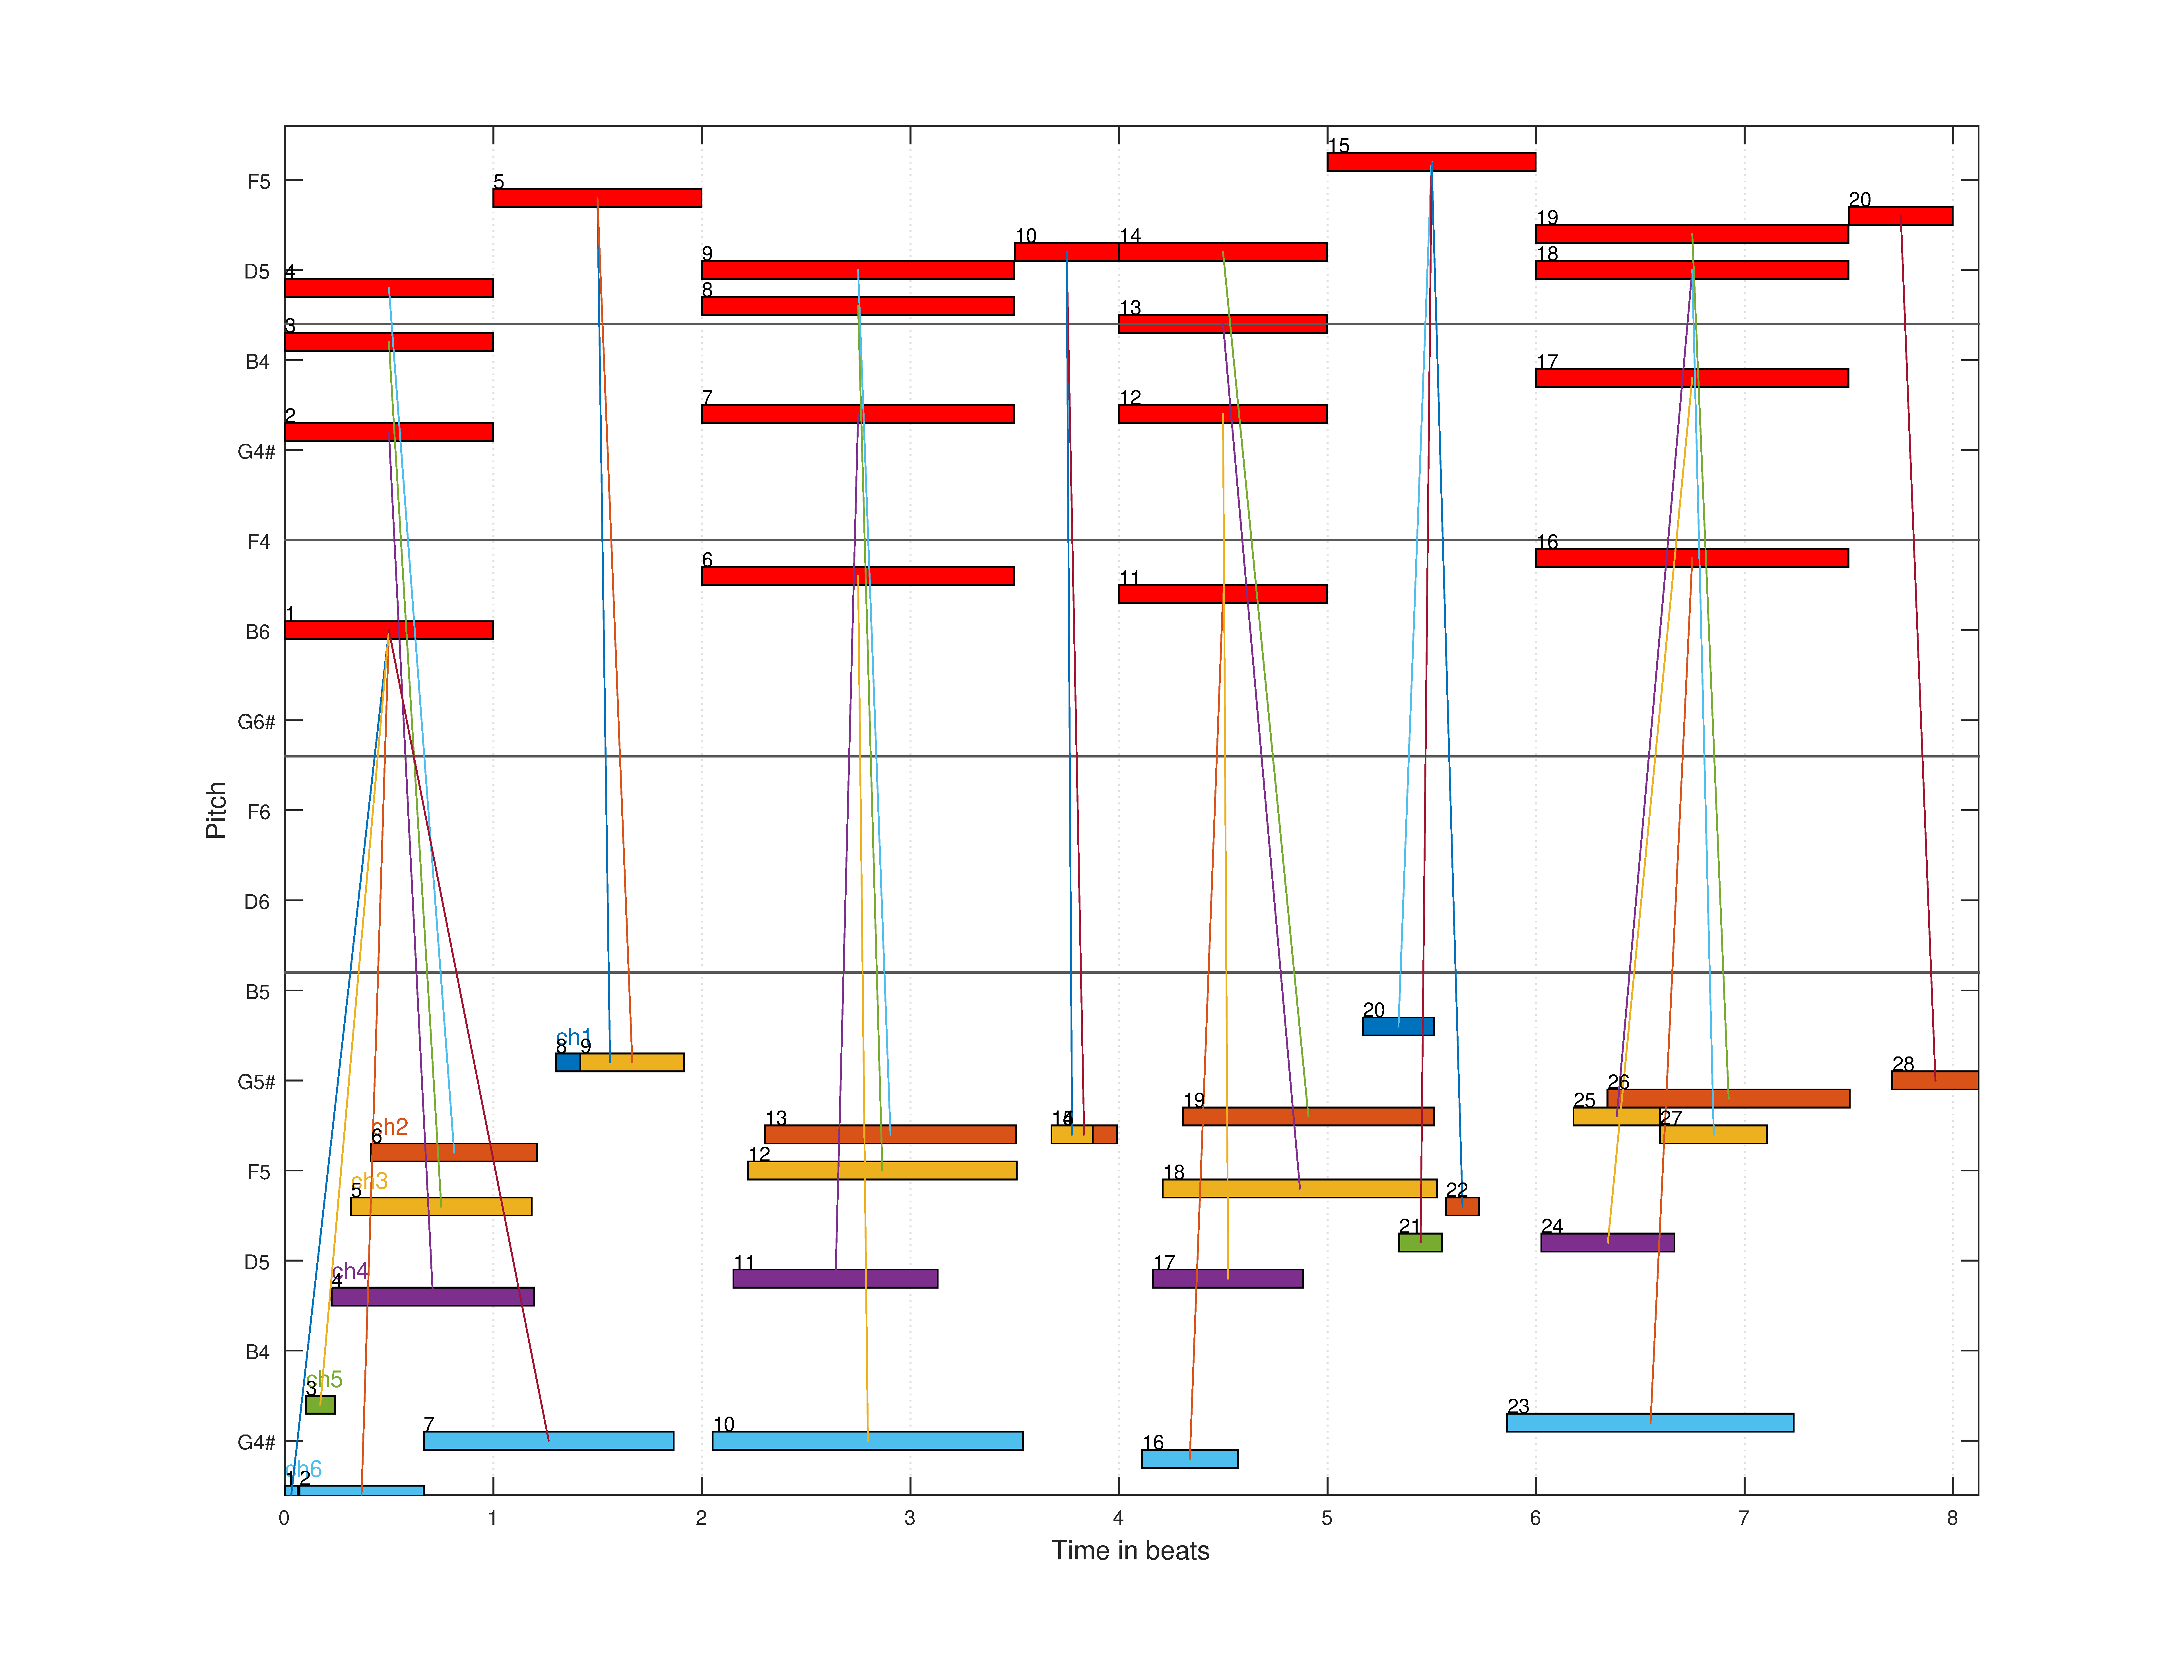
\includegraphics[width=0.7\textwidth]{Figures/Darn_8b_corrected.pdf}
\end{figure}
\subsection{Performance actions}
\section{Machine Learning modelling}
\cleardoublepage

